\chapter{Project Overview}

\vspace*{1cm}

This chapter presents the general structure of the project, its objectives, the
model used, the dataset selected, and the main workflow followed during the
implementation. The project is centered on the optimization and compression of a
Small Language Model for Edge AI applications.

\section{Project Objective}

The main objective of this project is to fine-tune a compact language model and
compare several optimization algorithms in order to study their impact on model
quality and computational efficiency. The work does not only focus on improving
the training loss, but also on evaluating practical constraints such as memory
usage, inference latency, model size, and training speed.

\vspace*{0.5cm}

This objective is important because Edge AI environments require efficient models
that can run under limited hardware resources. A model that performs well but
requires high memory, long inference time, or high energy consumption may not be
suitable for deployment on edge devices.

\section{Selected Model}

The model selected for this project is \texttt{google/flan-t5-small}. This model
is a small version of the FLAN-T5 family and is designed for text-to-text tasks.
It is already instruction-tuned, which means that it can understand and respond to
natural language instructions.

\vspace*{0.5cm}

The choice of \texttt{flan-t5-small} is suitable for this project because it
provides a compromise between language understanding capability and computational
cost. Its relatively small size makes it more realistic for optimization and
future compression experiments compared with larger language models.

\section{Dataset Used}

The dataset used in the project is \texttt{yahma/alpaca-cleaned}. It is an
instruction-following dataset composed of examples containing instructions,
optional inputs, and expected outputs. This type of data is appropriate for
fine-tuning an instruction-following language model.

\vspace*{0.5cm}

The dataset was processed into three subsets:

\begin{itemize}
    \item Training set: 2000 examples.
    \item Validation set: 500 examples.
    \item Test set: 500 examples.
\end{itemize}

\vspace*{0.5cm}

The processed files are stored in the \texttt{data/processed/} directory in both
\texttt{CSV} and \texttt{JSONL} formats. The training pipeline uses the
\texttt{source\_text} column as model input and the \texttt{target\_text} column
as the expected output.

\section{General Workflow}

The project workflow is divided into several main steps. First, the dataset is
loaded, cleaned, shuffled, and transformed into an instruction-tuning format.
Second, the tokenizer and the model are loaded from Hugging Face. Third, the
training script fine-tunes the model using the selected optimizer. Finally, the
trained model and the evaluation metrics are saved for comparison.

\vspace*{0.5cm}

The general workflow can be summarized as follows:

\begin{figure}[H]
    \centering
    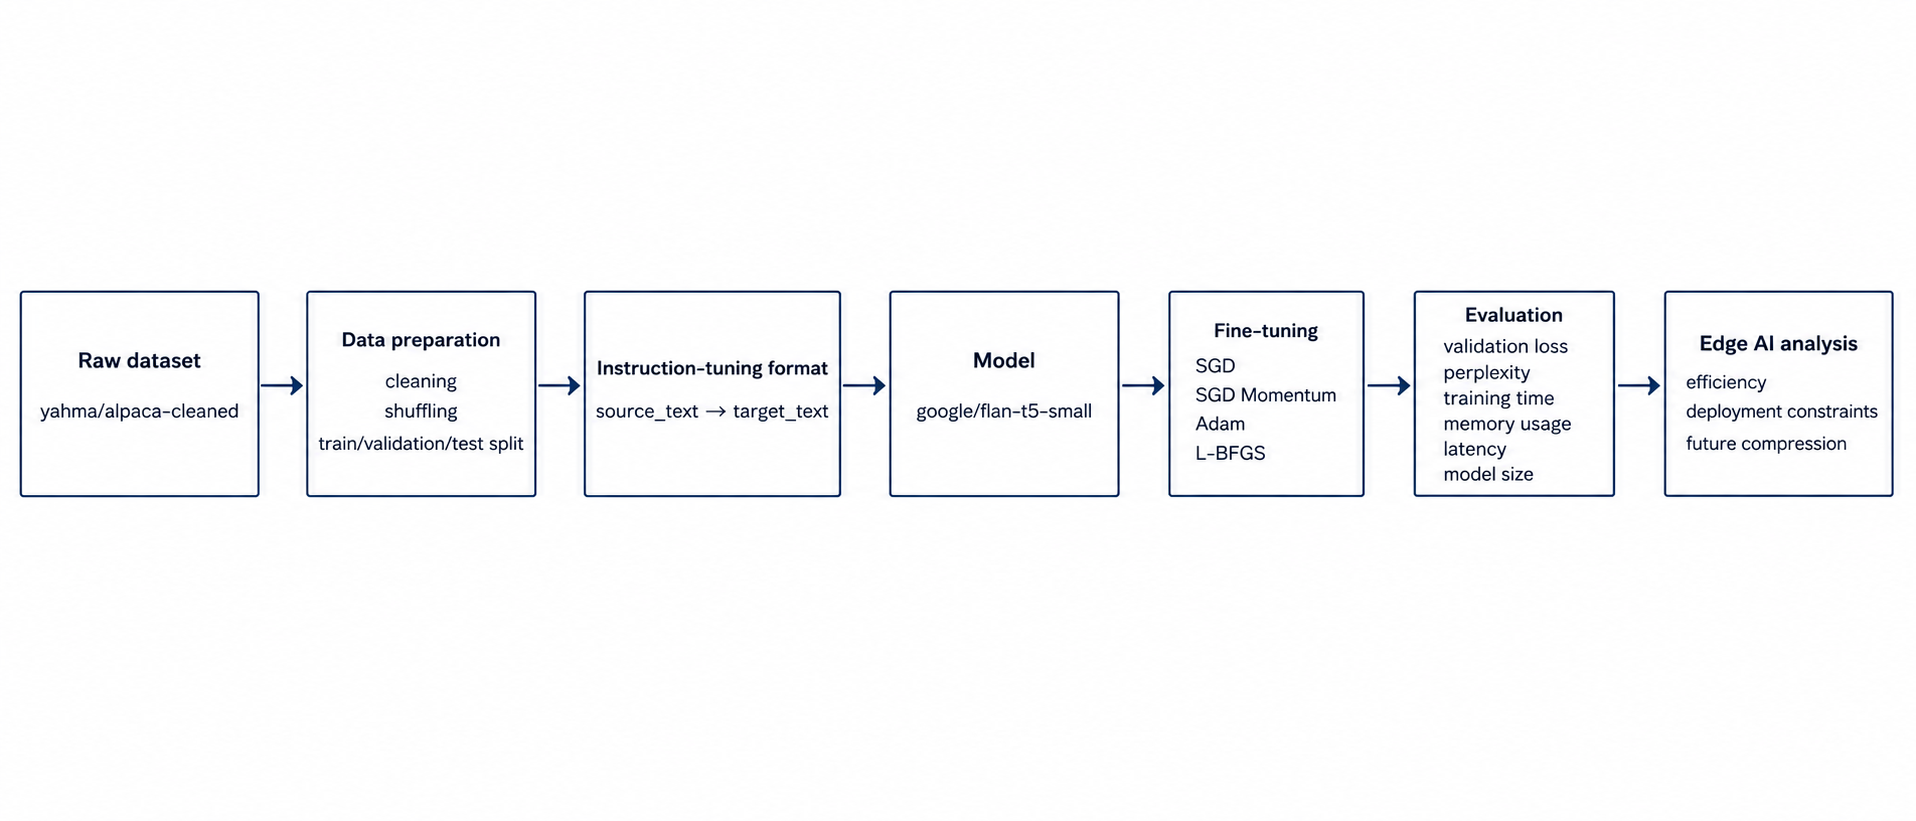
\includegraphics[width=\textwidth]{chapters/images/project_flow.png}
    \caption{General workflow of the project.}
    \label{fig:project_workflow}
\end{figure}

\begin{enumerate}
    \item Load the configuration from \texttt{config.yaml}.
    \item Prepare the instruction-tuning dataset.
    \item Load \texttt{google/flan-t5-small} and its tokenizer.
    \item Fine-tune the model using one optimizer.
    \item Save the trained model.
    \item Compute and save evaluation metrics.
    \item Compare the optimizers according to Edge AI criteria.
\end{enumerate}

\section{Project Structure}

The implementation is organized into several folders. The \texttt{src/} folder
contains the source code for data preparation, model loading, tokenization,
training, optimizer selection, and metrics computation. The \texttt{data/}
folder contains the processed dataset. The \texttt{results/} folder is reserved
for trained models, logs, checkpoints, and metrics. The \texttt{docs/} folder
contains project documentation.

\vspace*{0.5cm}

The main source files used in the project are:

\begin{itemize}
    \item \texttt{prepare\_data.py}: prepares the dataset.
    \item \texttt{train.py}: runs the fine-tuning process.
    \item \texttt{optimizers.py}: defines the optimizer selection logic.
    \item \texttt{model\_utils.py}: loads and saves the model.
    \item \texttt{tokenizer\_utils.py}: handles tokenization.
    \item \texttt{metrics.py}: computes training and inference metrics.
    \item \texttt{training\_config.py}: stores training parameters.
\end{itemize}

\section{Expected Outcome}

At the end of the project, each optimizer should produce a trained model and a
metrics file. These outputs make it possible to compare the optimization
algorithms and identify which one provides the best compromise between model
performance and resource efficiency.

\vspace*{0.5cm}

This comparison prepares the project for a future compression phase, where the
fine-tuned models can be further optimized using techniques such as quantization
or pruning.
